
%
\documentclass[conference]{IEEEtran}
% Add the compsoc option for Computer Society conferences.
%
% If IEEEtran.cls has not been installed into the LaTeX system files,
% manually specify the path to it like:








% *** GRAPHICS RELATED PACKAGES ***
%
\ifCLASSINFOpdf
  % \usepackage[pdftex]{graphicx}
  % declare the path(s) where your graphic files are
  % \graphicspath{{../pdf/}{../jpeg/}}
  % and their extensions so you won't have to specify these with
  % every instance of \includegraphics
  % \DeclareGraphicsExtensions{.pdf,.jpeg,.png}
\else
  % or other class option (dvipsone, dvipdf, if not using dvips). graphicx
  % will default to the driver specified in the system graphics.cfg if no
  % driver is specified.
  % \usepackage[dvips]{graphicx}
  % declare the path(s) where your graphic files are
  % \graphicspath{{../eps/}}
  % and their extensions so you won't have to specify these with
  % every instance of \includegraphics
  % \DeclareGraphicsExtensions{.eps}
\fi
% graphicx was written by David Carlisle and Sebastian Rahtz. It is










\hyphenation{op-tical net-works semi-conduc-tor}
\usepackage[T1]{fontenc}
\usepackage{amsmath}
\usepackage{amssymb}
\usepackage{exscale}
\usepackage{relsize}
\usepackage{mathenv}
\usepackage{cite}
\usepackage{url}
\usepackage{amsmath}
\usepackage{graphicx}
\usepackage{float}
\usepackage{algorithmicx,algorithm}
\usepackage[noend]{algpseudocode}
\usepackage{multirow}
\bibliographystyle{IEEEtran}

\begin{document}

%\title{A Dynamic Cluster-based Wireless Network for Software Defined Coalition }
\title{A Cluster-based Software Defined Network at Mobile Tactical Edge}

\author{\IEEEauthorblockN{Geng Li, Yang Richard Yang}
\IEEEauthorblockA{Computer Science Department, Yale University\\
New Haven, CT 06511
}
}



\maketitle

%\begin{abstract}
%%\boldmath

%\end{abstract}
%\IEEEpeerreviewmaketitle



\section{Introduction}
\label{s1}
On the battlefield, military operations are mostly organized on the basis of coalitions, each of which involves a set of resources, including troops, vehicles, computation and storage. To extend Software Defined Networking (SDN)'s concept of separating the control and data plane, researchers proposed Software Defined Coalitions (SDC), where the resources within an enclave (e.g., a battalion, a squad) are observed and controlled by a single logical controller. Obviously, SDC can achieve the benefit of optimized policies by the global network view and centralized control.

Nevertheless, due to the particularities of the network in tactical edge, three critical issues are not well resolved in such an SDC-enabled centralized network. (1)~\emph{Robustness} is incapable of being retained if the connectivity to controller gets lost, which happens inevitably and constantly in battles.(2)~\emph{Security} is hardly protected as once the enemy gets the controller, the entire management over the network is lost. (3)~\emph{Scalability} is not well established because the network cannot react agilely towards nodes getting lost or army being reorganized. Further more, some other challenges also remain in the centralized SDC network, such as high overhead, slow network updating and low efficiency.

In this paper, we propose a cluster-based architecture for SDC wireless networks, where an enclave can be dynamically partitioned into multiple administrative domains and the cluster head with SDN control functions manages the flow packet forwarding in each domain. Specifically, it is allowed that \textbf{multiple cluster domains belong to different organizations} (i.e. units of a coalition partner or even across coalition partners). Clustering algorithms and inter-domain protocols are also designed in our work accordingly. With the network management controlled by SDN, the centralized routing decisions and policies have better global optimality and lower convergence time in comparison with distributed protocols (e.g., ad-hoc). Furthermore, the clustered SDC networks not only adapt the high dynamics, but also meet the requirements for military coalition systems.
\section{Related Work}
Openflow is originally designed for wired network, but for wireless mesh networks
ad-hoc cluster. self-organization.  no dynamic. no central controller. no hierarchy. only sensor, SDC multiple resources.
differs from state of the art solutions as it provides
\section{Cluster-based SDC Wireless Networks}
\label{s2}
In this section, we introduce the architecture of the cluster-based wireless network for SDC, discuss its use cases, and describe parts of our research contents and future work.
\subsection{Network Architecture}
In this paper, we focus on the intra-enclave network, and the coordination between enclaves is not in the scope of our study. Without loss of generality, we consider a single enclave consisting of a logical controller (core controller) and a number of moving nodes, which could be the controllable mobile assets such as UAVs, robots, vehicles, etc. Nodes communicate with the controller and each other via wireless signals. In respect that nodes are distributed at geographically dispersed locations and the transmission power varies among different type of assets, one node can only reach a certain number of neighbors. To ensure the security and reliability of the control plane, we consider the out-of-band control, where the controller as a superior base station, operates in a special control channel and communicates with nodes directly. The controller is connected to all the nodes supposedly, and can determine the best routing, forwarding decisions, then inserts these decisions into nodes' flow tables. However, due to the frequent link failures in war conditions, nodes may lose the connection to controller and the topology may change dynamically.

In the proposed clustered-SDC network, an enclave can adaptively fragment into temporary clusters in responding to dynamics. Each cluster as an autonomous system is called an \textbf{SDN Domain}. A certain node in the cluster serves as the cluster head (CH), which is a wireless controller with SDN functionalities and in charge of the management of the whole cluster, a.k.a. domain~\cite{olivier2015sdn}. If there are links between domains, the border nodes then act as gateways to aggregate and transmit the data from the belonging domain to the other domains. A domain is therefore composed of a CH, gateways and cluster members as shown in Fig.~\ref{usecase}.
\begin{itemize}
\item Cluster Head (CH): is the coordinator of the domain.
\item Gateway Node (GN): is a bridge node between different domains.
\item Cluster Members: are the groups of nodes in a domain together with their gateways.
\end{itemize}

Every CH acts as a temporary base station within its domain, and utilizes OpenFlow communication protocol to control flow packet forwarding of its members~\cite{dely2011openflow,luo2012sensor}. Once the topology in a cluster changes, the CH needs to update the local database and generate new routing policies. The connection between CHs and the core controller is dispensable. If the CH is capable of connecting to the core, then we define this cluster as an \textbf{anchored cluster}, and if not, the cluster is a \textbf{free cluster}. In an anchored cluster, the powerful core controller in communication with other SDN domains can determine the global routing policies and the CH just needs to relay this control plane information by transparent transmission. Meanwhile in a free cluster, the CH has to compute the local routing decisions and border policies by itself. When a CH is disabled (link broken or asset lost), the entire domain becomes inaccessible temporarily. Based on self-stabilizing clustering for wireless ad-hoc networks, a new CH can be selected promptly.

Cluster member nodes do not make routing decisions, they only forward and drop packets according to the rules set by their CH or the controller. Member nodes may maintain the connections with local CH and core controller (or other physical controllers) simultaneously. In case that the CH fails, another controller can take over to avoid system failures, increasing trustworthiness and fault tolerance. In Openflow specifications version 1.3, two modes of operations for multiple controllers in the SDN are identified: Equal interaction and Master/Slave interaction. These options are both feasible in the OpenDaylight project, making the cluster-based SDC networks well supported.
\subsection{Use Cases}
There are four basic use cases in the clustered SDC network in responding to the high dynamics on battlefields, and each of them is treated as independent. So all kinds of the topology mutation can be abstracted as one of the four cases or a combination of a couple of them.
\begin{figure}
\centering
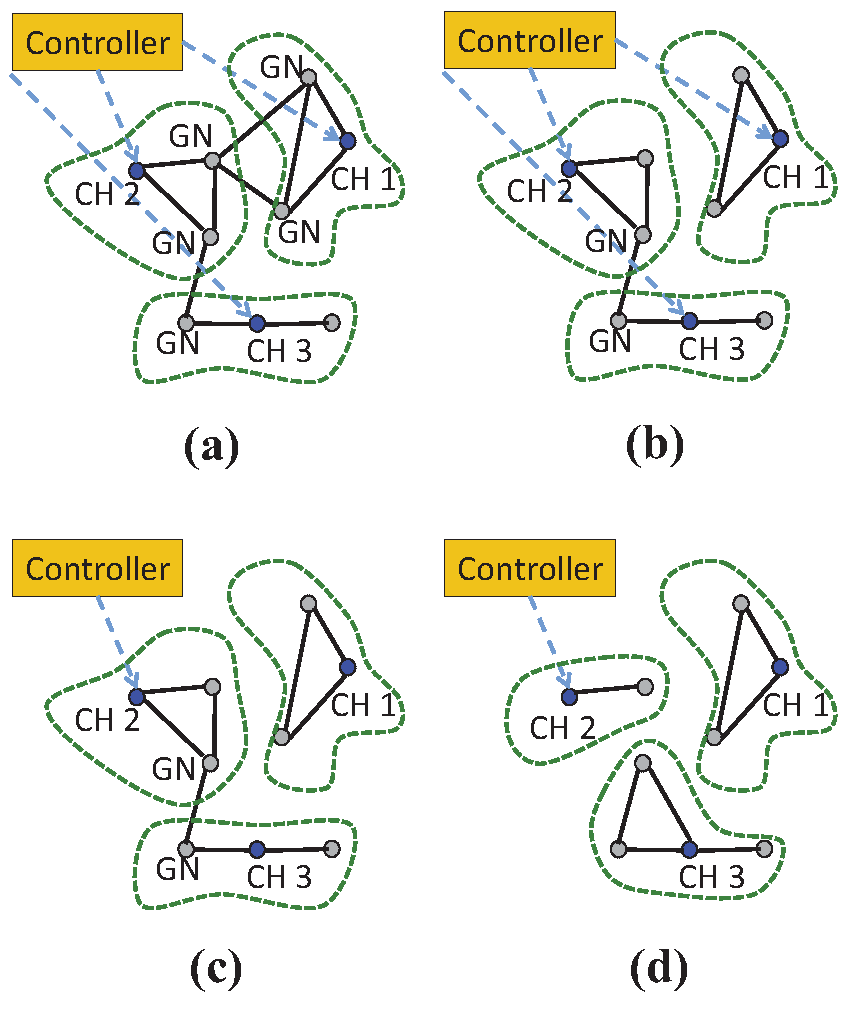
\includegraphics[width=3.2in]{usecase}
\caption{The use cases of cluster-based SDC wireless networks, where CHs represent cluster heads and GNs represent gateway nodes. (a) Anchored Clustering. (b) Anchored Re-clustering. (c) Free Clustering. (d) Free Re-clustering.}
\label{usecase}
\end{figure}
\subsubsection{Anchored Clustering}
As the enclave moves on, some of the nodes may lose the connectivity to the core controller, while some may not. Therefore, according to the link status of the topology and the connections to controller, a part of moving nodes can form into anchored clusters, whose CHs still maintain the connectivity to the core (such as CH 1, CH 2 and CH 3 in Fig.~\ref{usecase}(a)). As it's taken literally, the control of this cluster is ``anchored'' to the core controller. The network information is collected, aggregated and reported by the CHs, which makes this clustering approach efficient. The border nodes serve as gateways (GNs) to exchange data between clusters.
\subsubsection{Anchored Re-clustering}
When link failures happen inside an anchored cluster or on GNs, the core controller can be well aware of the changes and update new routing rules which are relayed by the CH. Like the example in Fig.~\ref{usecase}(b), the links between cluster 1 and 2 are broken, then the previous GNs are adjusted into simple cluster members.
\subsubsection{Free Clustering}
For sometimes CHs may also lose the connectivity to controller (as CH 1 and CH 3 in Fig.~\ref{usecase}(c)), or there is no one able to reach the controller in a certain range of area. The nodes thus end up with free clusters, where the self-stabilizing clustering protocols for ad-hoc networks are adopted. The CH can be selected by k-clustering solution, which specifies each node to be located at a most distance of k from the CH~\cite{caron2010self}.
\subsubsection{Free Re-clustering}
When the link state involved in free clusters is getting changed, the re-clustering mechanism is employed locally. Specifically, after member nodes report the new state, the CH can generate new routing policies and install them into its members, like the example of CH 3 in Fig.~\ref{usecase}(d).
\section{Clustering Algorithms}
In clustered SDC networks, splitting a single domain network into multiple-clusters is desirable. In this study, we will propose and design a series of clustering algorithms that choose the controller (CH) placement based on the following criterions sequentially.
\subsection{Topology Graph}
\begin{figure}
\centering
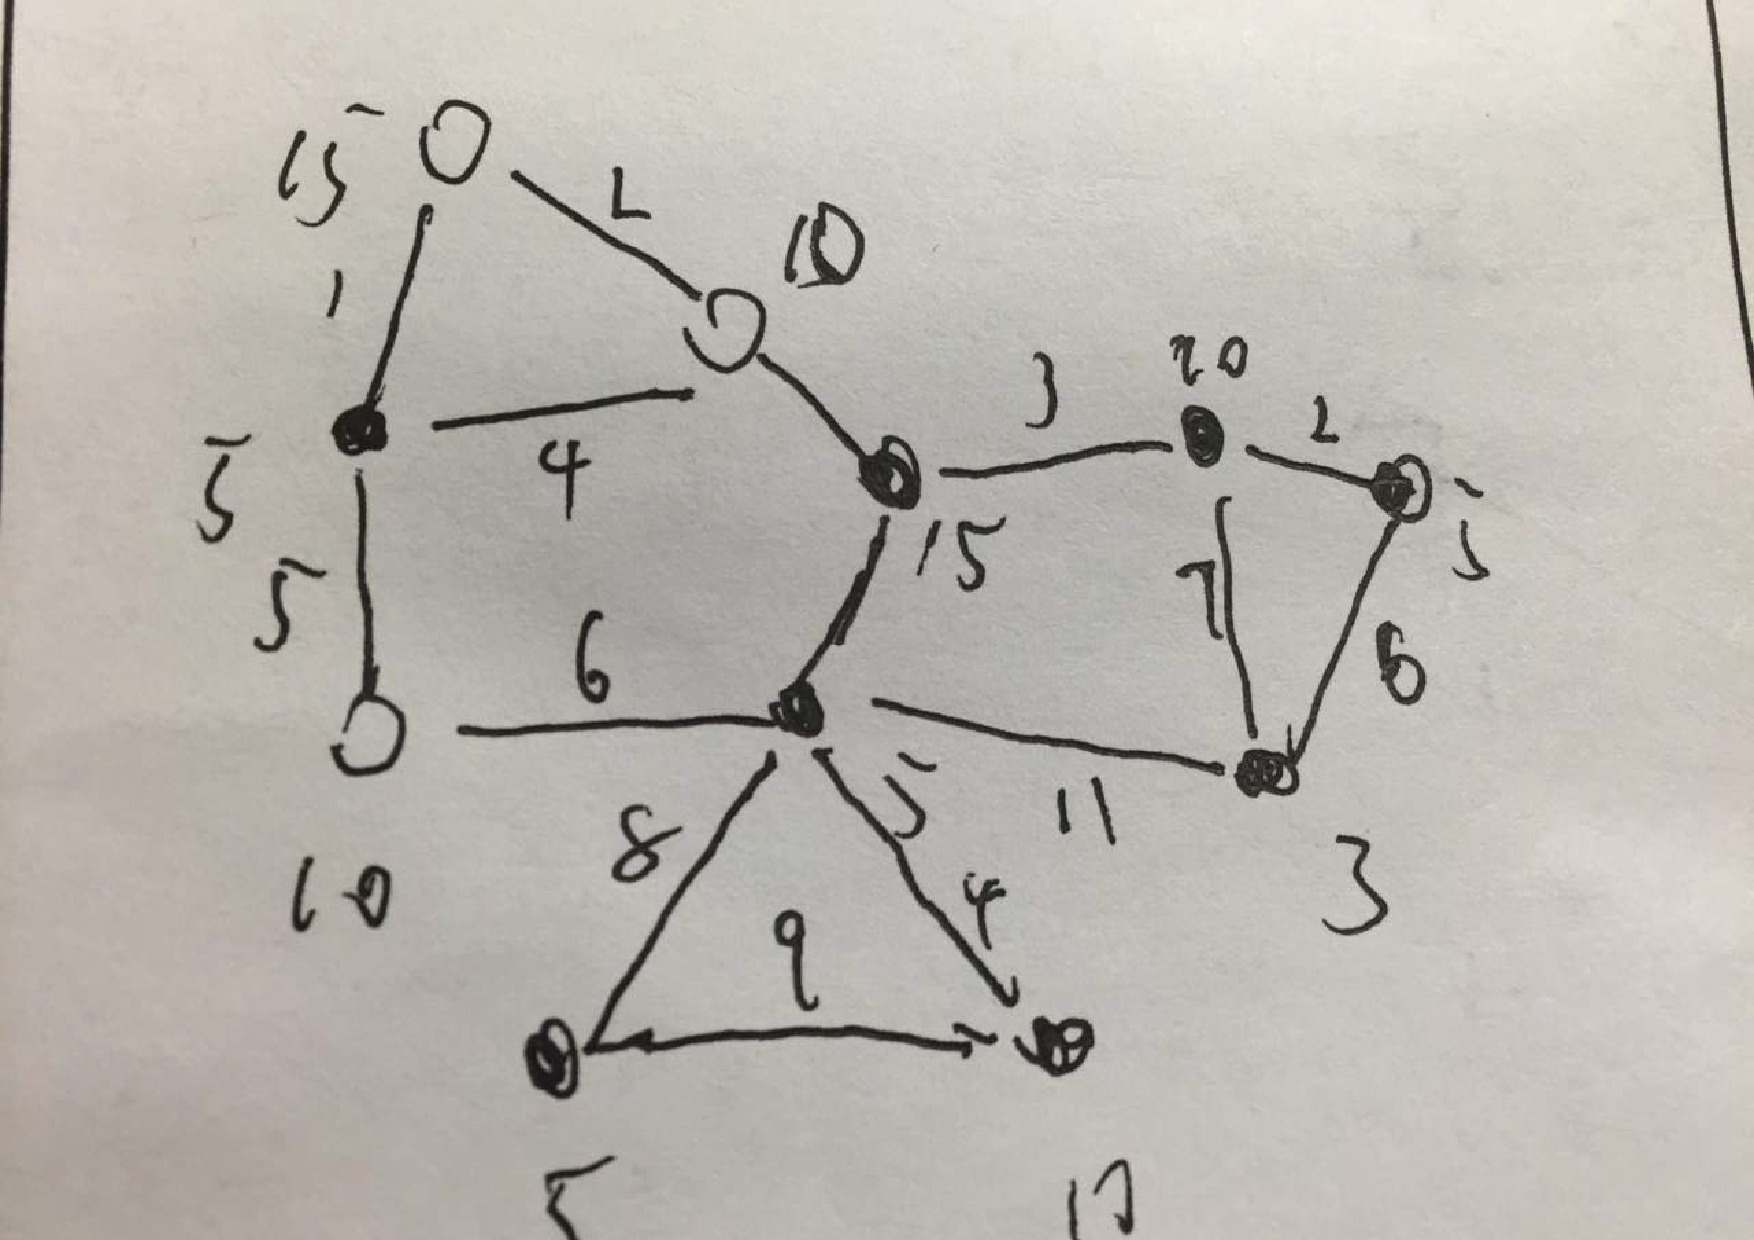
\includegraphics[width=2.4in]{model}
\caption{Network topology, where solid dots indicate the nodes that maintain the connectivity to the core controller, and hollow ones indicate the nodes without connectivity to the core. Edge weights represent the link costs.}
\label{model}
\end{figure}
In our model, the network is represented by a graph $G(V,E)$, which consists of $N$ nodes and $M$ edges. The set of vertexes is denoted as $V = \{v_1,...,v_N\}$, and the distance $d(i,j)$ is the minimum length (i.e., number of hops) of all paths connecting $v_i$ and $v_j$ in $G$. In this way, the corresponding vertex-cut, vertex-connectivity, edge-cut and edge-connectivity of $G$ can be obtained respectively.

There are two kinds of nods in the topology. One is the nodes that maintain the connectivity to the core controller (solid nodes). The other one is the nodes without connectivity to the core controller (hollow nodes).

The edge weight $w_{i,j}=w_{j,i}$ ($i,j \in \{ 1,2,...,N\}$) represents the link cost which is related to propagation attenuation of wireless signal. There is also a vale $p_i$ on each node which is quantized as the terminal capability. On the one hand, this value $p_i$ can reflect the transmission gain. As the example shown in Fig.~\ref{manvehicle}(a), although the link costs of $w_{1,3}$ and $w_{2,3}$ are the same, but the transmission powers from a vehicle and a hand-hold terminal are different, which results in the difference of received signal strength power for the node 3. We can simply use $w_{i,j}-p_i$ to indicate the received signal power for node $j$ from node $i$. On the other hand, $p_i$ is also an indicator of processing capability for a terminal. For example, the received powers for node 3 from the warfighter and the vehicle happen to be equal. But node 3 still prefers the vehicle as a CH rather than the warfighter, because the vehicle CH can provide a faster calculating speed, a larger number of supported connections, hence a better system performance.
\begin{figure}
\centering
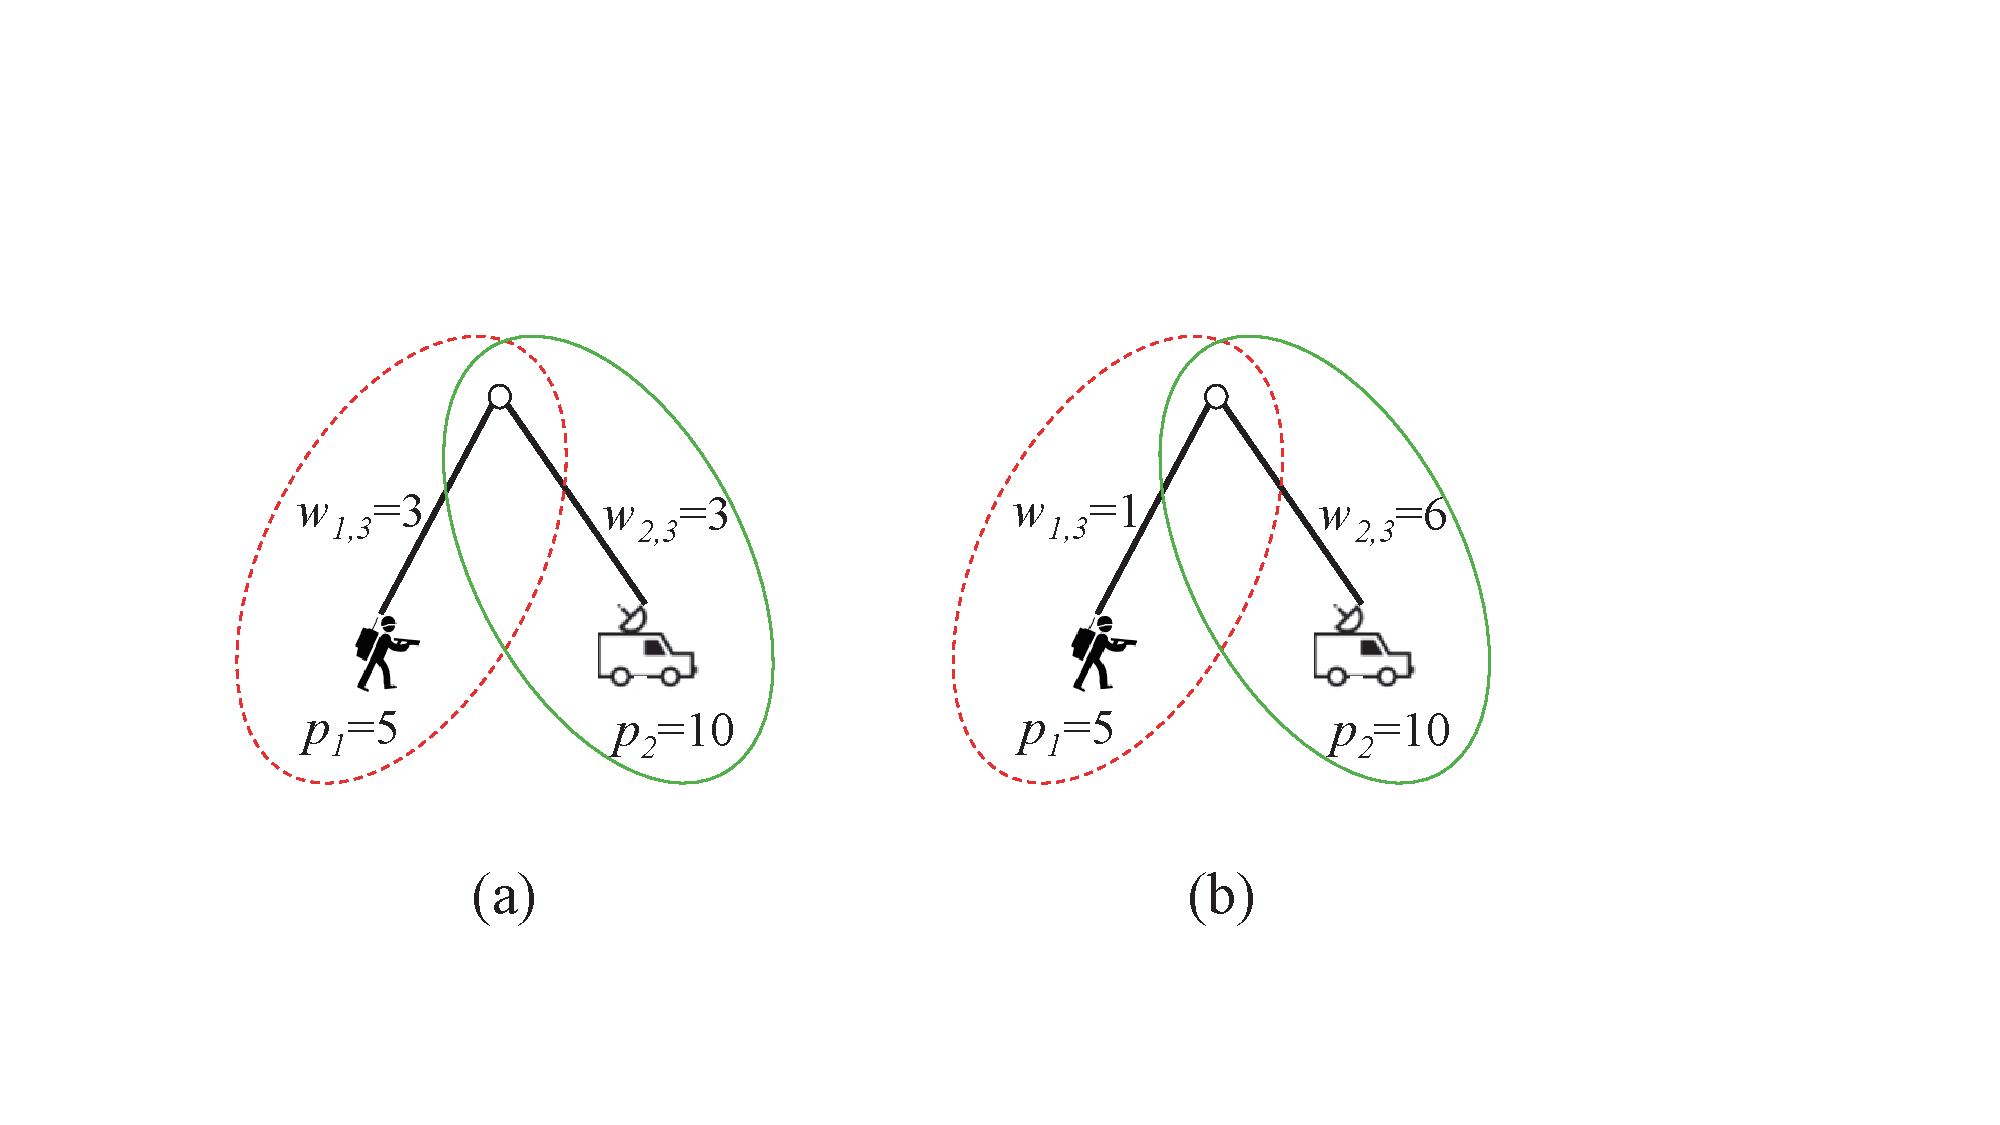
\includegraphics[width=2.4in]{manvehicle}
\caption{Illustration of the terminal capability $p_i$ impacting on the clustering results}
\label{manvehicle}
\end{figure}

\subsection{Problem Formulation}

The problem of splitting a network is a clustering problem. Since our goal is to reduce the signal power loss and improve the system performance, the objective of the problem is to minimize the total cost from each node to its corresponding CH. We use the network topology as input. (There are two kinds of nods in the network. One is the nodes that maintain the connectivity to the core controller (solid nodes). The other one is the nodes without connectivity to the core controller (hollow nodes).) The aim is to determine which nodes belong to a same cluster and which node to be the cluster head (CH) in this cluster. The problem has the following constraints.
\begin{enumerate}
\item The number of clusters is limited. This constraints the total bandwidth that the controller communicates with the CH. 
\item Only the nodes that maintain the connectivity to the core controller can be the CH of a cluster. This constraint can reduce the commnication cost to the core controller.
\item *The weight of an edge (one hop) in a cluster is limited. This ensures that the packet can be decoded correctly.
\end{enumerate}

\begin{table}[htbp]
\centering
\begin{tabular}{|c||c|}
\hline
Symbol & Decription\\
\hline
$k$ & The number of clusters.\\
\hline
$CM$ & The cost matrix of the network.\\
\hline
$CR$ & The result of clustering.\\
\hline
$r_i$ & The $ith$ node belongs to which cluster.\\
\hline
$CH$ & The cluster head in the result.\\
\hline
$ch_j$ & The cluster head of the $jth$ cluster.\\
\hline
$v_{jk}$ & The $kth$ node in the $jth$ cluster.\\
\hline
$C_t$ & The total cost.\\
\hline
\end{tabular}
\caption{Key notations in problem formulation}
\label{notations}
\end{table} 

\subsection{algorithm}
%\subsection{Priority Vector}
%Anchored clusters are logically controlled by the core controller, which leads to a better global optimality comparing with free clusters. Therefore the nodes connecting to the core controller have a higher priority to be selected as CHs. In the meantime, the wireless terminals with different processing capability can provide different performance when selected as CHs (e.g., a vehicle is more likely the CH than a warfighter). As a result, we introduce a priority vector $P=(p_i)^N$ into the clustering model, and the vector element $p_i$ for each node is calculated according to the terminal capability and the connectivity to the core.

To solve the problem, we use a clustering algorithm for weighted graph. The distance between each node is neccessary in k-means, so the cost between each node is calculated first using Dijkstra's algorithm. All the cost between every node can be represent by a cost matrix. Table\ref{cost_matrix} shows an example of cost matrix. (Brief intruduction of cost matrix?).

The input of the algorithm is the cost matrix $CM$ and the number of cluster $K$. We first choose the initial cluster head randomly. Then iteration are used to get the final cluster. There are two steps in each iteration: clustering and finding the CHs. To avoid that too many nodes gather in one cluster, load balancing has been intruduced in clusering step. As the CH must be the solid node, we find the nearest solid node of each CH as the final CHs after the iteration.

\begin{table}[htbp]
\centering
\begin{tabular}{|c|c|c|c|c|c|}
\hline
 & $n_1$ & $n_2$ & $n_3$ & ... & $n_n$ \\
\hline
$n_1$ & 5 & 7 & 3 & ... & 2 \\
\hline
$n_2$ & 3 & 4 & 1 & ... & 5 \\
\hline
$n_3$ & 5 & 1 & 3 & ... & 8 \\
\hline
... & \multicolumn{5}{c|}{...} \\
\hline
$n_n$ & 6 & 4 & 7 & ... & 10 \\
\hline
\end{tabular}
\caption{Cost matrix}
\label{cost_matrix}
\end{table}

\begin{algorithm}[htbp]
\caption{Clustering Alogrithm for Weighted Graph}
{\bf Input:}\\
\hspace*{0.1in}Num of clusters: $K$;\\
\hspace*{0.1in}Cost matrix: $CM$;\\
{\bf Output:}\\
\hspace*{0.1in}Clustering result: $CR=\left \{ r_{i}, 1 \leqslant i \leqslant N \right \}$;\\
\hspace*{0.1in}Clustering head: $CH=\left \{ ch_{j}, 1 \leqslant j \leqslant K \right \}$;\\
\hspace*{0.1in}Total cost: $C_t$;\\
{\bf Initialization:}\\
\hspace*{0.1in}Random choose the initial $CH$;
\begin{algorithmic}[1]
\State $his \leftarrow null$
\While{$CH \neq his$}
    \State $his \leftarrow CH$
    \For {each node $v_i$}
        \State Find $ch_j$ which has the minimal cost to connect
        \State $r_i \leftarrow j$
    \EndFor
    \State Perform load banlancing
    \For {each cluster $C_j$}
        \State Find the node $v_{jk} \in C_j$ which has the minimal total cost to connect
        \State $ch_j \leftarrow v_{jk}$
    \EndFor
\EndWhile
\State $CH \leftarrow findNearestSolidNode(CH)$
\State \Return $CR, CH$
\end{algorithmic}
\end{algorithm}

\subsection{Asymptotical Updating}
In order to limit the updating overhead and maintain continuous accessability, we expect a smooth and asymptotical updating process when the network is re-clustered in our design. So we further leverage a filter $X_i(t)$ upon the priority variable $p_i$ to retain the previous CHs as possible, unless crucial links are broken.
\section{Inter-domain Protocols}
As we illustrated before, a cluster is an administrative domain, whose members are under the control of a single administration (i.e., the cluster head). Accordingly, the inter-domain coordination, such as peering, routing offerings and load balancing issues, should be addressed by inter-domain protocols. For anchored clusters, with a hierarchy-like control plane structure, each CH can build a local network view, and exchange the local domain view with other CHs through a WE-Bridge~\cite{lin2014we}. But for free clusters, or the clusters belonging to different organizations, the control plane is distributed, so a CH has to employ neighbor-discovering process and exchange aggregated network-wide information with neighbor domains via border GNs (BGP and DISCO~\cite{phemius2014disco} for instance). Different inter-domain routing protocols can be deployed concurrently by D-BGP~\cite{sambasivanbootstrapping}, which  supports evolvability to new protocols. In the particular case that there is only one node in the cluster, it is hence degraded into an ad-hoc network, and OLSR routing protocol in MANET can be well applied.

\section{SIMULATION}
The performance of the proposed algorithm is close to the theoritcal optimal value.

computation complexity

campare with other cluster algorithm

\begin{figure}[htbp]
  \centering
  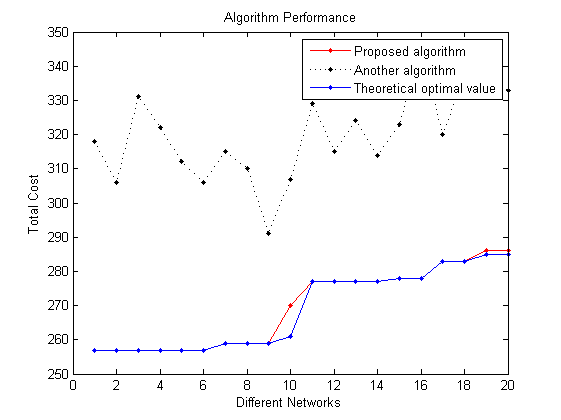
\includegraphics[width=0.35\textwidth]{figures/k2}
  \caption{Clustering Result (k=2)}\label{fig:k2}
  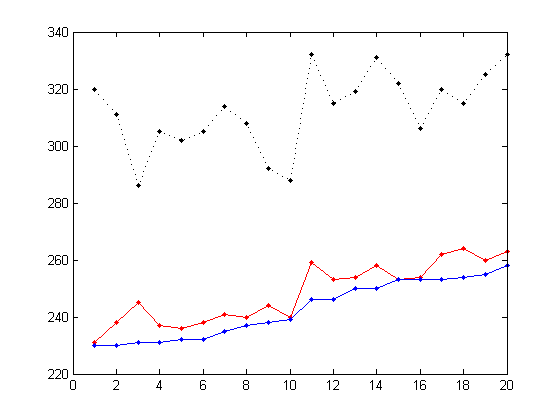
\includegraphics[width=0.35\textwidth]{figures/k3}
  \caption{Clustering Result (k=3)}\label{fig:k3}
\end{figure}

\section{CONLUSION}

\section*{Acknowledgment}
This research was sponsored by the U.S. Army Research Laboratory and the U.K. Ministry of Defence under Agreement Number W911NF-16-3-0001. The views and conclusions contained in this document are those of the authors and should not be interpreted as representing the official policies, either expressed or implied, of the U.S. Army Research Laboratory, the U.S. Government, the U.K. Ministry of Defence or the U.K. Government. The U.S. and U.K. Governments are authorized to reproduce and distribute reprints for Government purposes notwithstanding any copyright notation hereon. This statement may be placed either at the bottom of the first page or at the end of the paper.
\bibliography{my}

\end{document}


